% !TEX program = xelatex
% 주차별 발표 자료 템플릿
% 이 파일이 있는 폴더에서 xelatex로 두 번 빌드한다.
% 디자인 원본: ../../templates/weekly_presentation_template.tex
\documentclass[aspectratio=169,11pt]{beamer}

\usepackage{fontspec}
\usepackage{kotex}
\usepackage{graphicx}
\usepackage{tikz}
\usetikzlibrary{positioning}

% D2Coding을 저장소에 함께 넣어, 별도 설치 없이 같은 글꼴로 빌드한다.
\setmainfont{D2Coding-Regular.ttf}[Path=../../assets/fonts/,BoldFont={D2Coding-Bold.ttf}]
\setmainhangulfont{D2Coding-Regular.ttf}[Path=../../assets/fonts/,BoldFont={D2Coding-Bold.ttf}]
\setsansfont{D2Coding-Regular.ttf}[Path=../../assets/fonts/,BoldFont={D2Coding-Bold.ttf}]
\setsanshangulfont{D2Coding-Regular.ttf}[Path=../../assets/fonts/,BoldFont={D2Coding-Bold.ttf}]
\setmonofont{D2Coding-Regular.ttf}[Path=../../assets/fonts/,BoldFont={D2Coding-Bold.ttf}]

% University of Seoul identity color
\definecolor{UOSBlue}{HTML}{005EB8}
\definecolor{TextGray}{HTML}{303030}

\setbeamertemplate{navigation symbols}{}
\setbeamercolor{normal text}{fg=TextGray,bg=white}
\setbeamercolor{frametitle}{fg=UOSBlue,bg=white}
\setbeamercolor{title}{fg=white}
\setbeamercolor{structure}{fg=UOSBlue}
\setbeamertemplate{itemize item}{\color{UOSBlue}\small$\bullet$}
\setbeamertemplate{itemize subitem}{\color{UOSBlue}\scriptsize$\bullet$}
\setbeamertemplate{frametitle}{%
  \vspace{0.55cm}\hspace{0.48cm}\insertframetitle\par\vspace{0.12cm}}
\setbeamerfont{frametitle}{series=\bfseries,size=\LARGE}

% 기준 자료처럼 하단에 소속과 페이지 번호를 표시한다.
\setbeamertemplate{footline}{%
  \begin{tikzpicture}[remember picture,overlay]
    \node[anchor=south,inner sep=0pt] at ([yshift=0.52cm]current page.south)
      {
\includegraphics[width=2.64cm,trim=58bp 385bp 58bp 385bp,clip]{../../assets/uos-logo-horizontal.png}};
    \node[anchor=east,text=gray,font=\scriptsize]
      at ([xshift=-0.57cm,yshift=0.52cm]current page.south east) {\insertframenumber};
  \end{tikzpicture}%
  \vspace{0.38cm}}

\newcommand{\week}{LAB 1}
\newcommand{\course}{전자전기컴퓨터설계실험Ⅱ}
\newcommand{\topic}{Vivado 2026.1\\설치 매뉴얼}
\newcommand{\presenter}{이해리}
\newcommand{\presentationdate}{2026. 09. 07.}

\title{\course\\\week. \topic}
\author{\presenter}
\date{\presentationdate}


\newcommand{\screen}[2]{%
\begin{center}
\includegraphics[width=\linewidth,height=5.25cm,keepaspectratio]{assets/vivado-install/#1}\\[-0.05cm]
{\tiny\color{gray}#2}
\end{center}}
\newcommand{\source}[2]{\par\vspace{0.15cm}{\tiny\color{gray}출처: \href{#1}{#2}}}
\newcommand{\shotframe}[4]{%
\begin{frame}{#1}
\begin{columns}[c,onlytextwidth]
\begin{column}{0.64\textwidth}\screen{#2}{#3}\end{column}
\begin{column}{0.33\textwidth}\small #4\end{column}
\end{columns}
\end{frame}}

\begin{document}

% 표지
{\setbeamertemplate{footline}{}
\setbeamercolor{background canvas}{bg=UOSBlue}
\begin{frame}[plain]
  \begin{tikzpicture}[remember picture,overlay]
    \node[anchor=north west,inner sep=0pt,text=white,font=\bfseries\fontsize{27}{33}\selectfont,align=left]
      at ([xshift=1.53cm,yshift=-1.5cm]current page.north west) {\course\\\week. \topic};
    \node[anchor=south west,inner sep=0pt] at ([xshift=1.38cm,yshift=0.98cm]current page.south west)
      {
\includegraphics[width=1.45cm]{../../assets/uos-logo-white.png}};
    \node[anchor=south east,text=white,font=\small\bfseries,align=right]
      at ([xshift=-1.38cm,yshift=0.98cm]current page.south east)
      {\presentationdate\\\presenter};
  \end{tikzpicture}
\end{frame}}


\begin{frame}{설치 순서}
\begin{enumerate}
\item 설치 파일 다운로드
\item Vivado와 Spartan-7 디바이스 설치
\item 무료 BASIC 라이선스 발급·등록
\item 실행·부품 검색·XSim 파일 확인
\end{enumerate}
\vspace{0.4cm}
Windows 기준 안내이며, 설치는 수업 전에 완료한다.
\end{frame}

\begin{frame}{설치 전 준비}
\begin{itemize}
\item Windows PC와 AMD 계정을 준비한다.
\item 수업에서는 Vivado 2026.1과 Spartan-7을 사용한다.
\item 설치 화면의 필요 공간과 여유 공간을 비교한다.\\
다운로드·압축 해제에 사용할 공간도 확보한다.
\item 설치·드라이버 등록 중에는 권한 승인이 필요할 수 있다.\\
평소 VS Code를 항상 관리자 권한으로 실행할 필요는 없다.
\end{itemize}
\source{https://docs.amd.com/r/en-US/ug973-vivado-release-notes-install-license/Supported-Operating-Systems}{AMD UG973: Supported Operating Systems}
\end{frame}

\begin{frame}{2026.1 BASIC 라이선스}
\begin{itemize}
\item BASIC은 무료이며 Spartan-7을 지원한다.
\item 2026.1부터 무료 BASIC도 라이선스 파일을 발급·등록한다.
\item 라이선스는 12개월마다 갱신한다.
\item 구버전의 “무료 버전은 라이선스 파일이 필요 없다”는\\
안내를 그대로 적용하지 않는다.
\end{itemize}
\source{https://www.amd.com/en/products/software/adaptive-socs-and-fpgas/licensing-faq.html}{AMD Licensing FAQ}
\source{https://www.amd.com/en/products/software/adaptive-socs-and-fpgas/vivado/vivado-buy.html}{AMD Vivado: 디바이스별 라이선스 지원}
\end{frame}

\begin{frame}{1. 설치 파일 다운로드}
\begin{enumerate}
\item \href{https://www.amd.com/en/support/downloads/adaptive-socs-and-fpgas/development-tools/2026-1.html}{AMD 2026.1 다운로드 페이지}에 접속한다.
\item Windows Self Extracting Web Installer를 선택한다.
\item AMD 계정으로 로그인하고 설치 파일(\texttt{.exe})을 받는다.
\end{enumerate}
\vspace{0.25cm}
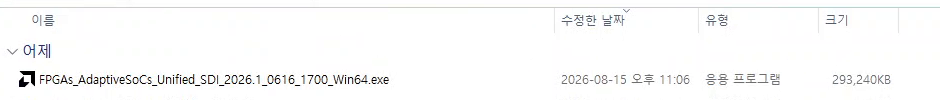
\includegraphics[width=\textwidth]{assets/vivado-install/01-installer-file.png}
\par{\tiny\color{gray}화면 A 18:20. 빌드 번호는 배포 시점에 따라 달라질 수 있다.\par}
\vspace{0.3cm}
\small Lab Edition은 장치 프로그래밍·디버깅용이다.\\
이번 수업에는 시뮬레이션·합성·구현이 가능한 전체 Vivado가 필요하다.
\end{frame}

\shotframe{2. 로그인과 설치 방식}{08-install-login.png}{화면 B 01:10 · 계정 입력 전}{
\begin{enumerate}
\item 설치 파일을 실행하고 압축 해제를 기다린다.
\item AMD 이메일·비밀번호를 입력한다.
\item \textbf{Download and Install Now}를 선택하고 Next를 누른다.
\end{enumerate}
\vspace{0.2cm}
Download Image는 설치 이미지만 받는 선택지다.
}

\shotframe{3. 제품 선택}{09-select-vivado.png}{화면 B 01:49}{
\textbf{Vivado}를 선택하고 Next를 누른다.
\vspace{0.4cm}
\par 이번 FPGA HDL 실습에서는 이 제품을 사용한다.
}

\shotframe{4. 도구와 드라이버}{10-install-options.png}{화면 B 01:55 · 디바이스는 다음 화면에서 확인}{
\begin{itemize}
\item Vivado의 필수 구성은 유지한다.
\item Model Composer 등 불필요한 추가 도구는 해제한다.
\item \textbf{Install Cable Drivers}를 확인한다.
\item \textbf{Acquire or Manage a License Key}를 확인한다.
\end{itemize}
{\footnotesize 드라이버 안내에 따라 Platform Cable USB를 분리한다.}
}

\shotframe{5. Spartan-7 선택}{11-device-selection.png}{화면 B 01:58 · 녹화에는 Virtex-7이 선택되어 있음}{
\begin{enumerate}
\item Devices의 \textbf{7 Series}를 펼친다.
\item \textbf{Spartan-7 FPGAs}를 선택한다.
\item 다른 디바이스 계열은 해제한다.
\item Selected Devices도 확인한다.
\end{enumerate}
\textbf{\color{UOSBlue}녹화의 Virtex-7 선택을 그대로 따라 하지 않는다.}
}

\shotframe{6. 약관 확인}{12-license-agreements.png}{화면 B 01:59 · 동의 전 화면}{
각 약관을 읽고 동의하는 항목의 \textbf{I Agree}를 선택한다.
\vspace{0.4cm}
\par 필요한 동의를 마치면 Next로 진행한다.
\vspace{0.4cm}
\par 약관 목록은 선택 구성에 따라 달라질 수 있다.
}

\shotframe{7. 설치 경로와 오류 확인}{13-destination-errors.png}{화면 B 02:12 · 오류 때문에 Next가 비활성화된 예시}{
설치 기준 경로 예:
\par\texttt{C:\textbackslash AMDDesignTools}
\vspace{0.3cm}
\begin{itemize}
\item 경로에는 공백을 넣지 않는다.
\item 필요 공간과 여유 공간을 비교한다.
\item 빨간 오류가 있으면 해결한 뒤 진행한다.
\end{itemize}
\textbf{이 화면은 설치 완료 화면이 아니다.}
}

\begin{frame}{설치 경로 화면의 두 오류}
\begin{itemize}
\item \textbf{There is not enough disk space}\\
녹화 당시 필요 공간은 71.3GB, 여유 공간은 50.37GB다.\\
Spartan-7 선택 후 요구량을 다시 확인하고, 부족하면\\
공간을 확보하거나 다른 드라이브를 사용한다.
\item \textbf{Program group entry ... already exists for 2026.1}\\
기존 설치의 시작 메뉴 그룹과 충돌한다. 재설치 필요 여부를\\
확인하고, 추가 설치 시 그룹 이름·생성 옵션을 조정한다.
\end{itemize}
\vspace{0.2cm}
\small 화면의 용량은 Virtex-7 선택 당시 값이다.\\
오류를 없애려고 기존 설치 폴더를 무작정 삭제하지 않는다.
\end{frame}

\begin{frame}{8. Summary 확인과 설치}
\begin{enumerate}
\item 오류를 해결한 뒤 Next로 진행한다.
\item Installation Summary에서 제품·디바이스·경로를 확인한다.
\item Install을 누르고 다운로드·설치 완료를 기다린다.
\item 완료 후 라이선스 발급·등록으로 진행한다.
\end{enumerate}
\vspace{0.25cm}
\small 기본 경로 예: \texttt{C:/AMDDesignTools/2026.1/Vivado}\\
설치 진행이 느리면 로그·네트워크·남은 공간을 먼저 확인한다.\\
진행 중인 설치를 여러 개 동시에 실행하지 않는다.
\source{https://docs.amd.com/r/en-US/ug973-vivado-release-notes-install-license/Run-the-Installation-File}{AMD UG973: Run the Installation File}
{\tiny\color{gray}9월 6일 녹화는 오류 화면까지다. 이후 설치 단계는 공식 절차를 따른다.}
\end{frame}

\shotframe{9. License Manager}{02-obtain-license.png}{화면 A 00:05}{
시작 메뉴에서\\
\textbf{Manage AMD Licenses}를 실행한다.
\begin{enumerate}
\item Obtain License
\item Get My Full or Purchased Certificate-Based License
\item Connect Now
\end{enumerate}
Purchased라는 표현이 있어도 무료 BASIC을 발급할 수 있다.
}

\shotframe{10. 무료 BASIC 선택}{03-basic-license.png}{화면 A 01:05}{
AMD 사이트에 로그인하고 본인 정보를 확인한다.
\begin{enumerate}
\item Create New Licenses
\item \textbf{Vivado Basic Tier License, Node Locked License}
\item \textbf{No Charge} 확인
\item Generate Node-Locked License
\end{enumerate}
평가판이나 구형 WebPACK과 구분한다.
}

\shotframe{11. 사용할 PC 지정}{04-node-license.png}{화면 A 01:30 · Host ID 선택 전}{
\begin{enumerate}
\item 제품이 Vivado Basic인지 확인한다.
\item Select a host에서 사용할 PC를 선택한다.
\item 목록에 없으면 Add a Host로 등록한다.
\end{enumerate}
Host ID는 License Manager의 \textbf{View Host Information}에서 확인한다.
}

\begin{frame}{12. 라이선스 파일 받기}
\begin{enumerate}
\item 사용할 PC의 Host ID와 선택 제품을 확인한다.
\item Next로 진행해 약관 확인과 발급을 마친다.
\item 이메일 또는 사이트의 Manage Licenses에서\\
발급된 \texttt{.lic} 파일을 받는다.
\end{enumerate}
\vspace{0.4cm}
Node-locked 라이선스는 지정한 PC에 연결된다.\\
다른 사람의 Host ID를 복사하지 않는다.
\vspace{0.25cm}
\par\textbf{계정 정보·Host ID·라이선스 파일은 공개 저장소에 올리지 않는다.}
\source{https://docs.amd.com/r/en-US/ug973-vivado-release-notes-install-license/Create-and-Generate-a-License-Key-File}{AMD UG973: Create and Generate a License Key File}
\end{frame}

\begin{frame}{13. 라이선스 등록}
\begin{enumerate}
\item License Manager에서 \textbf{Load License}를 선택한다.
\item \textbf{Copy License...}를 누르고 받은 \texttt{.lic} 파일을 연다.
\item 복사 완료 메시지를 확인한다.
\end{enumerate}
\vspace{0.25cm}
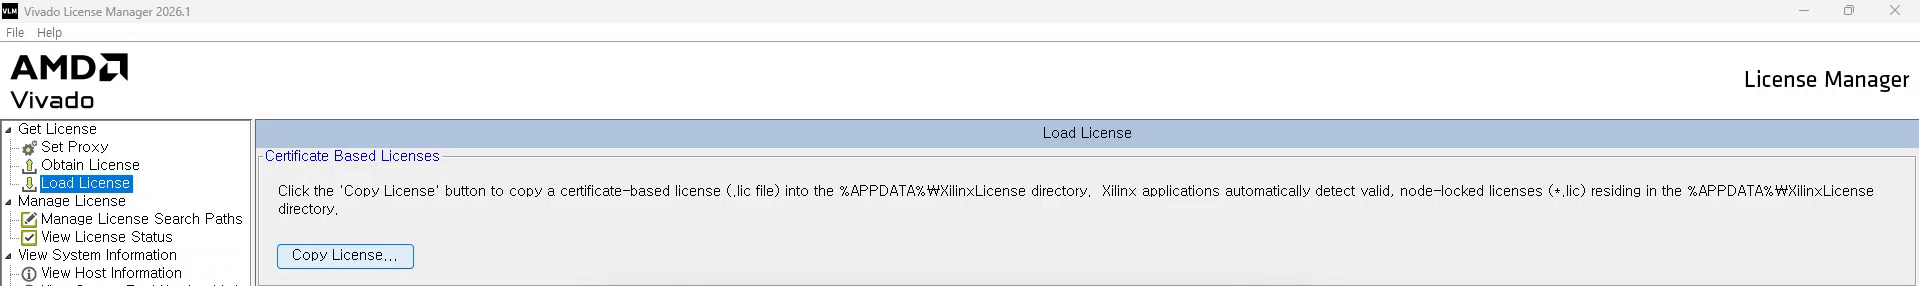
\includegraphics[width=\textwidth]{assets/vivado-install/05-load-license.png}
\par{\tiny\color{gray}화면 A 15:25 · 개인 폴더 목록을 제외한 상단 영역\par}
\vspace{0.15cm}
\small Windows 등록 위치: \texttt{\%APPDATA\%\textbackslash XilinxLicense}
\source{https://docs.amd.com/r/en-US/ug973-vivado-release-notes-install-license/Install-Certificate-Based-Node-Locked-License-Key-File}{AMD UG973: Install Certificate-Based Node-Locked License Key File}
\end{frame}

\begin{frame}{14. 라이선스 상태 확인}
\begin{itemize}
\item \textbf{View License Status}에서 BASIC 인식 여부를 확인한다.
\item 만료일과 \textbf{Host IDs Match}를 확인한다.
\item No라면 현재 PC의 Host ID와 발급 정보를 비교한다.
\item 호스트 정보가 다르면 AMD 사이트에서 정정·재발급한 뒤\\
새 파일을 등록한다. 라이선스 본문을 직접 수정하지 않는다.
\end{itemize}
\vspace{0.3cm}
\small 원본 영상 A 15:05에는 Host IDs Match가 No인 상태가 나온다.\\
BASIC이 목록에 있다는 것만으로 등록 성공을 판단하지 않는다.
\end{frame}

\shotframe{15. Vivado 실행}{06-vivado-basic.png}{화면 A 16:25}{
Vivado 2026.1을 실행한다.
\vspace{0.4cm}
\par 라이선스 오류 없이 시작 화면이 열리는지 확인한다.
\vspace{0.4cm}
\par 이 단계와 실제 보드 프로그래밍 검증은 별개다.
}

\shotframe{16. 확인용 프로젝트}{07-rtl-project.png}{화면 A 18:00}{
\begin{enumerate}
\item New Project를 누른다.
\item 이름과 저장 위치를 정한다.
\item \textbf{RTL Project}를 선택한다.
\item \textbf{Do not specify sources at this time}을 선택한다.
\end{enumerate}
}

\begin{frame}{17. Spartan-7 부품 검색}
\begin{enumerate}
\item 부품 선택 화면에서 \textbf{Parts} 탭을 연다.
\item 검색창에 \texttt{xc7s75fgga484-1}을 입력한다.
\item 해당 부품이 검색되는지 확인한다.
\end{enumerate}
\vspace{0.35cm}
\begin{itemize}
\item 검색되지 않으면 검색 필터와 Spartan-7 설치 여부를 확인한다.
\item 필요하면 설치 프로그램에서 디바이스 지원을 추가한다.
\end{itemize}
\vspace{0.2cm}
\small 부품 번호는 수업 신 장비 레거시 기준이다.\\
실제 보드 부품과 핀맵은 실험실 확인 결과를 따른다.
\end{frame}

\begin{frame}[fragile]{18. XSim 실행 파일 확인}
PowerShell에서 실행한다.
\begin{verbatim}
$vivadoBin = 'C:/AMDDesignTools/2026.1/Vivado/bin'
Test-Path "$vivadoBin/xvlog.bat"
Test-Path "$vivadoBin/xelab.bat"
Test-Path "$vivadoBin/xsim.bat"
\end{verbatim}
\begin{itemize}
\item 세 결과가 모두 \texttt{True}인지 확인한다.
\item 다른 위치에 설치했다면 위 경로와 배포 프로젝트의\\
\texttt{.vscode/tasks.json} 경로를 맞춘다.
\item 파일 존재 확인 뒤 실제 시뮬레이션·VCD 생성은\\
별도 조합회로 시뮬레이션 매뉴얼에서 진행한다.
\end{itemize}
\end{frame}

\shotframe{19. 환경 변수 설정 열기}{14-system-properties.png}{화면 C · 2026.09.07 실제 Windows 설정 화면}{
\begin{enumerate}
\item Windows 시작 메뉴에서 \textbf{시스템 환경 변수 편집}을 검색한다.
\item 시스템 속성의 \textbf{고급} 탭을 연다.
\item \textbf{환경 변수...}를 누른다.
\end{enumerate}
PATH는 명령 이름으로 실행 파일을 찾을 때 검색하는 폴더 목록이다.
}

\begin{frame}{20. 사용자 PATH에 Vivado 추가}
\begin{enumerate}
\item 위쪽 \textbf{사용자 변수}에서 \textbf{Path}를 선택하고 편집한다.
\item \textbf{새로 만들기}를 누르고 다음 폴더를 한 줄로 추가한다.
\end{enumerate}
\vspace{0.2cm}
\centering\texttt{C:\textbackslash AMDDesignTools\textbackslash 2026.1\textbackslash Vivado\textbackslash bin}
\par\vspace{0.25cm}
\raggedright
\begin{itemize}
\item 기존 항목을 지우거나 전체 값을 덮어쓰지 않는다.
\item 다른 위치에 설치했다면 실제 Vivado의 bin 폴더를 넣는다.
\item 이미 같은 항목이 있으면 중복 추가하지 않는다.
\item 열린 설정 창의 확인을 눌러 저장한다.
\end{itemize}
\end{frame}

\begin{frame}[fragile]{21. PATH 적용 확인}
VS Code와 터미널 앱을 완전히 종료한 뒤 다시 실행한다.
\begin{verbatim}
where.exe xvlog.bat
where.exe xelab.bat
where.exe xsim.bat
xsim.bat -version
\end{verbatim}
\begin{itemize}
\item 출력 경로가 등록한 Vivado 2026.1의 bin인지 확인한다.
\item 버전 출력 예: \texttt{Vivado Simulator v2026.1}
\item 계속 찾지 못하면 로그아웃·로그인 후 다시 확인한다.
\end{itemize}
\small PATH 등록 후에는 전체 경로 없이 도구를 호출할 수 있다.\\
프로젝트 task가 절대 경로를 사용한다면 그 설정도 따로 확인한다.
\end{frame}

\begin{frame}{설치 후 문제 해결}
\begin{itemize}
\item \textbf{Hardware Manager만 사용 가능}\\
Lab Edition만 설치했는지 확인한다.
\item \textbf{라이선스가 없다는 메시지}\\
2026.1 BASIC 파일의 등록 여부와 만료일을 확인한다.
\item \textbf{VS Code task가 도구를 찾지 못함}\\
실제 설치 경로와 tasks.json의 vivadoBin을 비교한다.\\
slang-server가 XSim 실행 파일을 대신하지는 않는다.
\end{itemize}
\vspace{0.25cm}
\small 질문할 때는 오류 메시지 전체·실행 단계·Vivado 버전을 제시한다.\\
계정 정보·라이선스 내용·Host ID는 가린다.
\end{frame}

\begin{frame}{설치 후 문제 해결: 한글 이름}
\begin{itemize}
\item \textbf{사용자명·장치 이름에 한글이 포함된 경우}\\
Vivado와 관련 도구가 정상 작동하지 않을 수 있다.
\item PowerShell에서 \texttt{whoami}를 실행해 이름을 확인한다.\\
로컬 계정은 \texttt{장치이름\textbackslash 사용자명} 형태로 출력된다.\\
장치 이름만 따로 확인하려면 \texttt{hostname}을 실행한다.
\item 한글 장치 이름은 영문으로 변경하고 재부팅한다.\\
한글 사용자명은 영문 이름의 새 Windows 계정으로 해결한다.
\item 계정의 표시 이름만 바꿔도 사용자 폴더 경로는 남을 수 있다.\\
기존 사용자 폴더의 이름을 탐색기에서 직접 바꾸지 않는다.
\end{itemize}
\vspace{0.25cm}
\textbf{설치 후에도 해결할 수 있다.} 문제가 생기면 이름부터 확인한다.
\end{frame}

\begin{frame}{설치 완료 기준}
\begin{enumerate}
\item Vivado 2026.1이 라이선스 오류 없이 열린다.
\item BASIC 라이선스의 만료일과 Host ID 일치를 확인했다.
\item \texttt{xc7s75fgga484-1} 부품을 검색할 수 있다.
\item XSim 실행 파일 세 개가 설치 경로에 있다.
\item 사용자 PATH에 Vivado bin을 등록하고 버전 출력을 확인했다.
\end{enumerate}
\vspace{0.4cm}
다음 매뉴얼: VS Code 확장 설치, 조합회로 시뮬레이션\\
\small JTAG 연결·비트스트림 다운로드는 실험실 보드 확인 후 진행한다.
\end{frame}

\begin{frame}{공식 문서}
\small
\begin{itemize}
\item \href{https://www.amd.com/en/support/downloads/adaptive-socs-and-fpgas/development-tools/2026-1.html}{AMD 2026.1 다운로드 및 제품 설명}
\item \href{https://docs.amd.com/r/en-US/ug973-vivado-release-notes-install-license/Run-the-Installation-File}{UG973: 설치 파일 실행과 설치 순서}
\item \href{https://docs.amd.com/r/en-US/ug973-vivado-release-notes-install-license/Install-Cable-Drivers}{UG973: 케이블 드라이버 설치}
\item \href{https://www.amd.com/en/products/software/adaptive-socs-and-fpgas/licensing-faq.html}{AMD Licensing FAQ: 2026.1 BASIC 정책}
\item \href{https://docs.amd.com/r/en-US/ug973-vivado-release-notes-install-license/Managing-Licenses-with-the-Vivado-License-Manager}{UG973: Vivado License Manager}
\item \href{https://docs.amd.com/r/en-US/ug973-vivado-release-notes-install-license/Create-and-Generate-a-License-Key-File}{UG973: 라이선스 발급과 Host ID}
\item \href{https://docs.amd.com/r/en-US/ug973-vivado-release-notes-install-license/Install-Certificate-Based-Node-Locked-License-Key-File}{UG973: Node-locked 라이선스 등록}
\end{itemize}
\vspace{0.2cm}
각 항목은 공식 페이지로 연결된다. 정책 확인일: 2026.09.07.
\end{frame}

\begin{frame}{화면 출처}
\small
\textbf{화면 A: 2026-08-16 13-44-25.mp4}
\begin{itemize}
\item 18:20 설치 파일 / 00:05 License Manager
\item 01:05 BASIC 선택 / 01:30 Host ID 선택 전
\item 15:25 Copy License / 16:25 BASIC 시작 / 18:00 RTL Project
\end{itemize}
\vspace{0.15cm}
\textbf{화면 B: 2026-09-06 23-56-46.mp4}
\begin{itemize}
\item 01:10 로그인 / 01:49 제품 선택 / 01:55 도구 구성
\item 01:58 디바이스 목록 / 01:59 약관 / 02:12 경로 오류
\end{itemize}
\vspace{0.15cm}
{\footnotesize 담당자 제공 녹화에서 화면 13장을 추출했다.\\
개인정보가 있는 주변 영역은 제외하고 설치·라이선스 창만 사용했다.}
\end{frame}

\begin{frame}{PATH 설정 화면 출처}
\begin{itemize}
\item 화면 C는 2026.09.07에 Windows 시스템 속성을 열어\\
직접 캡처한 화면이다.
\item 사용자 PATH에는 Vivado 2026.1의 bin 폴더를 추가한다.
\item 사용자마다 기존 PATH 항목과 설치 위치가 다를 수 있다.
\end{itemize}
\end{frame}
\end{document}
